%%%%%%%%%%%%%%%%%%%%%%%%%%%%%%%%%%%%%%%%%%%%

%%%%%%%%%%%%%%%%%%%%%%%%%%%%%%%%%%%%%%%%%%%%
% Class options                            %
%%%%%%%%%%%%%%%%%%%%%%%%%%%%%%%%%%%%%%%%%%%%
% Orientation:                             %
% portrait (default), landscape            %
%                                          %
% Paper size:                              %
% a0paper (default), a1paper, a2paper,     %
% a3paper, a4paper, a5paper, a6paper       %
%                                          %
% Language:                                %
% english (default), norsk                 %
%%%%%%%%%%%%%%%%%%%%%%%%%%%%%%%%%%%%%%%%%%%%
\documentclass{uibposter}


\usepackage{lipsum}                                % Dummy text
\usepackage[figwidth = 0.98\linewidth]{todonotes}  % Dummy image (and more!)
\usepackage[absolute, overlay]{textpos}
\usepackage{varwidth}
\DeclareUnicodeCharacter{200B}{ }% Figure placement
\setlength{\TPHorizModule}{\paperwidth}
\setlength{\TPVertModule}{\paperheight}


\title{Title}
\author
{%
    First Author
    \and
    Second Author
}
%% Optional:
\institute
{
    Department of mathematics -- University of Bergen
}


% Or:
%\institute{Contact information}


%% Remove footline:
%\setbeamertemplate{footline}{}


\begin{document}

\begin{textblock}{0.5}(0.038, 0.055)
    \color{white}
    \sffamily
    \textbf{Ingress}
    \\
Should contain the essence of the content. What is this poster about? What did you find? The ingress must be short, clear and no more than three lines!
\end{textblock}

\begin{frame}

\begin{columns}
\begin{column}{0.5\textwidth - 1.5cm}
    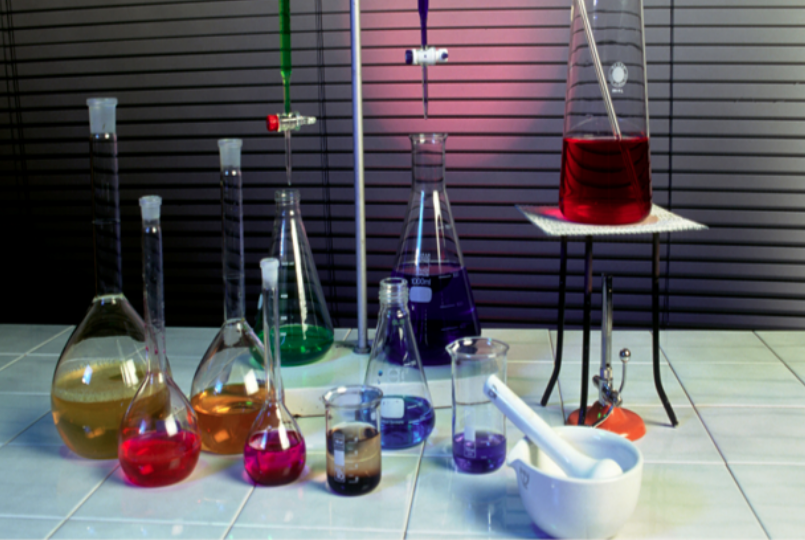
\includegraphics[width = \textwidth]{uibposter-images/bilde1.png}
    \vspace{0.5cm}

    \begin{column}{0.5\textwidth - 1.5cm}
        \textbf{Abstract}
\vspace{0.5cm}

Use this section to clarify the scope of the presentation. Choose only ONE essential concept to address in the poster and write a concise abstract that communicates what you have learned about this one concept and how it relates to a larger picture of your field.
\vspace{0.2cm}

This abstract should transmit the important point of your poster to the (typical) viewer who only reads the abstract and glances at the figures.
\vspace{0.2cm}

A poster must convey your basic message within two to three minutes. It should also engage the interest of the viewer so that they are willing to invest more of their time in you and your work.
\vspace{0.2cm}

In this section the font-size should be bigger than the rest of the presentation.
\vspace{0.2cm}

After reading the heading, the ingress and the first paragraph the visitor should be able to determine whether this is within his or her field of interest!
    \end{column}
    \begin{column}{0.5\textwidth - 1.5cm}
        \textbf{The presentation}
\vspace{0.5cm}

        Choose a short title (!)
\vspace{0.5cm}

        Use a smaller font for ingress and the poster author(s), and an even smaller one for associated institutional information (and abbreviate this — no one needs your street address).
\vspace{0.2cm}

        Use first names in the list of poster authors and add e-mail information for the lead author.
\vspace{0.5cm}

        \textbf{Text}
\vspace{0.5cm}

        Keep text to an absolute minimum. Write what you think is the absolute minimum, then force yourself to cut it in half.  Continually remind yourself "There is ALWAYS too much text in a poster."
        \vspace{0.5cm}

        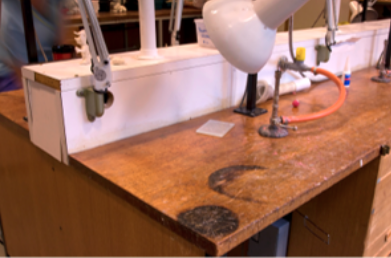
\includegraphics[width = \textwidth]{uibposter-images/bilde2.png}
        \vspace{0.5cm}

        \textbf{Graphics and images}
\vspace{0.5cm}

        A good way to structure a poster is to choose the graphics first, then write the “story” and arrange the spatial flow of the poster around them.
    \end{column}
\end{column}

\begin{column}{0.5\textwidth - 1.5cm}
\begin{column}{0.5\textwidth - 1.5cm}
\vspace*{-25.5cm}

    Images must be of high quality and in 1:1 scale (If the physical space it occupies is 15cm wide the image should have the same width). The  resolution should be 150dpi minimum. Smaller images may look fine on screen, but they become blurred when printed.


    \vspace{1.cm}

    \textbf{Readability}
\vspace{0.5cm}

    If something is easy to read, it is more likely to be read. Here are some guidelines:

\vspace{0.5cm}

    \textbf{Use black type on a white background.}
    \vspace{0.2cm}

    Intensely colored or “busy” backgrounds draw attention from the content and make it difficult to read.
\vspace{0.5cm}

    \textbf{Design simple flow paths.}
    \vspace{0.2cm}

    Complex paths from one element to another make it hard for the reader to follow the logical flow of your ideas. Disorganized posters reflect badly on your scientific thinking.
\vspace{0.5cm}

    \textbf{Use subheadings}
    \vspace{0.2cm}

    Descriptive subheadings make it easy for the reader to follow the logical flow of your content.
\vspace{0.5cm}

    \textbf{Double-space all text}
    \vspace{0.2cm}

    except for acknowledgments and references. Minimum font size (for content) should be 18pt.

    (The font size above is 36pt. With narrow columns like this a smaller font size (like 32pt) would be better.)
\vspace{0.5cm}

    \textbf{Use left-justification,}
    \vspace{0.2cm}

    shown to be easiest to read.
\vspace{0.5cm}

    \textbf{Use a sans-serif font}
    \vspace{0.2cm}

    Arial or Myriad are fonts specified by UiBs graphic profile. They are easier to read than serif fonts like Times New Roman.
\vspace{0.2cm}

    Be font consistent throughout the poster.
\vspace{0.2cm}

    Be consistent also when using text elements like \textbf{bold}, \textit{emphasis} and \underline{underline}.
\end{column}
\begin{column}{0.5\textwidth - 1.5cm}
\vspace*{-25.5cm}

    \textbf{Things to avoid}
\vspace{0.5cm}

    Do not use colorful backgrounds with super-imposed text, low-resolution images or L O N G lines of text.
        \vspace{1.5cm}

    \fbox{\small\begin{varwidth}{\textwidth}Do not use boxes like this unless they are necessary. This box is used to present content relating to the illustration below.\end{varwidth}}
    \vspace{1.5cm}

    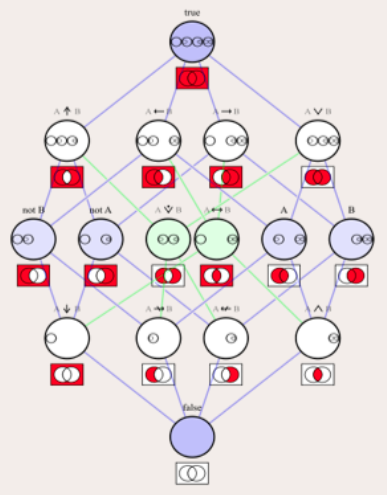
\includegraphics[width = \textwidth]{uibposter-images/bilde3.png}

    \textbf{Logos}

    Leave out unnecessary institutional “brands” or logos. The only logo used in this template is the UiB logo signalizing that this poster reflects research carried out at this institution.
\vspace{0.2cm}

    A research group may have members from various institutions and receive funding from different sources. This should be stated in the acknowledgment section unless you are bound by contract to include the logo.
\vspace{0.2cm}

    Including a variety of logos only add to visual confusion!
    \vspace{5cm}

    {\scriptsize
    \textbf{REFERENCES}

    Lorem ipsum dolor sit amet, consectetuer adipiscing elit, sed diam nonummy nibh euismod tincidunt ut laoreet dolore magna aliquam erat volutpat.

    Ut wisi enim ad minim veniam, quis nostrud exerci tation ullamcorper suscipit lobortis nisl ut aliquip ex ea commodo consequat. Duis autem vel eum iriure dolor in hendrerit in vulputate velit esse

    }
\end{column}
\end{column}
\end{columns}





\end{frame}
\end{document}
